
%%%%%%%%%%%%%%%%%%%%%%%%%%%%%%%%%%%%%%%%%%%%%%%%%%%%%%%%%%%%
%%%%%%%%%%%%%%%%%%%%%%% preamble %%%%%%%%%%%%%%%%%%%%%%%%%%%
%%%%%%%%%%%%%%%%%%%%%%%%%%%%%%%%%%%%%%%%%%%%%%%%%%%%%%%%%%%%

\documentclass[10pt,letterpaper]{article}

\usepackage{opex3}
\usepackage{times}
\usepackage{graphicx}
\graphicspath{{./images/}}
\usepackage{epstopdf}
\usepackage{amsmath}
\usepackage{amssymb}
\usepackage{url}
\usepackage{bm}
\usepackage{enumerate}
\usepackage[]{todonotes} % Add option [disable] to hide all todo notes.
\usepackage{xfrac}
\usepackage{paralist}
\usepackage{cite}
\usepackage{soul}
\usepackage{layouts}

%\usepackage{ae} %%for Computer Modern fonts

\usepackage{hyperref}
\hypersetup{pdfborder={0 0 0}}

%
% subfiles is useful for having the abstract (and possible other
% sections/chapters) as separate files.
%
\usepackage{subfiles}

\usepackage[]{siunitx}

%
% The cleveref package seems very cool but currently it doesn't support hebrew
% (babel) very well, so I just use if for single references.
% As a work around I redefine the number definition as suggested in:
% http://tex.stackexchange.com/questions/118235/using-the-cleveref-package-with-hebrew-and-babel
%
\usepackage[capitalise,poorman]{cleveref}
\crefname{section}{Sec.}{Secs.}
\Crefname{section}{Section}{Sections}
\makeatletter
\def\@@number#1{#1}
\makeatother

\DeclareMathAlphabet\mathbfcal{OMS}{cmsy}{b}{n}


%
% Some new commands I use in this text
%
% Note:
% Nice curly font is {\bm{\mathcal{D}}}
%
\newcommand{\Grad}[1]{\bm{\triangledown_{#1}}}
\newcommand{\abbrev}[1]{\rm{#1}}
\newcommand{\argmin}{\mathrm{arg}\min}
\newcommand{\curly}[1]{\left\{#1\right\}}
\newcommand{\roundy}[1]{\left(#1\right)}
\newcommand{\recty}[1]{\left[#1\right]}
\newcommand{\PartDeriv}[2]{\frac{\partial{#1}}{\partial{#2}}}
\newcommand{\vect}[1]{\bm{#1}}
\newcommand{\mat}[1]{\bm{#1}}
\newcommand{\transpose}[1]{{#1}^\intercal}
\newcommand{\derivsym}[1]{\,d{#1}}
\newcommand{\yoavcomment}[1]{}
\renewcommand{\yoavcomment}[1]{#1} % Comment to remove images
\newcommand{\fix}[2]{\st{#1}\hl{#2}}

%
% Used symbols (only partial for now...)
%
\newcommand{\OpSphere}{\mathbfcal{S}}
\newcommand{\OpRot}{\mathbfcal{R}}
\newcommand{\OpDistance}{\bm{D}}
\newcommand{\OpCumsum}{\mathbfcal{C}}
\newcommand{\OpInt}{\mathbfcal{I}}
\newcommand{\OpCamera}{\mathbfcal{P}}
\newcommand{\MaskSun}{\mathbfcal{M}}
\newcommand{\Laplacian}{\mathbfcal{L}}
\newcommand{\OpDiag}[1]{\mathbb{D}\left\{#1\right\}}
\newcommand{\DistSet}{\mathcal{C}}
\newcommand{\DistUnknown}{\vect{n}}
\newcommand{\DistEstimated}{\hat{\vect{n}}}
\newcommand{\CostFunc}[1]{E(#1)}

%
% For the title
%
\newcommand\authnote[1]{\textsuperscript{\normalfont#1}}
\newcommand\affilnote[1]{\textsuperscript{\normalfont#1}}
\providecommand\textsuperscript[1]{$^{#1}$}

%%%%%%%%%%%%%%%%%%%%%%%%%%%%%%%%%%%%%%%%%%%%%%%%%%%%%%%%%%%%
%%%%%%%%%%%%%%%%%%%%%%% begin %%%%%%%%%%%%%%%%%%%%%%%%%%%%%%
%%%%%%%%%%%%%%%%%%%%%%%%%%%%%%%%%%%%%%%%%%%%%%%%%%%%%%%%%%%%

\begin{document}
%\printinunitsof{in}\prntlen{\linewidth}

%%%%%%%%%%%%%%%%%%%%%%%%%%%%%%%%%%%%%%%%%%%%%%%%%%%%%%%%%%%%
%%%%%%%%%%%%%%%%%% title page information %%%%%%%%%%%%%%%%%%
%%%%%%%%%%%%%%%%%%%%%%%%%%%%%%%%%%%%%%%%%%%%%%%%%%%%%%%%%%%%

\title{Multi sky-view\\ 3D aerosol distribution recovery}

\author{Amit~Aides,\authnote{1*} Yoav~Y.~Schechner,\authnote{1}
  Vadim~Holodovsky,\authnote{1} Michael~J.~Garay\authnote{2} and Anthony~B.~Davis\authnote{2}}

\address{\affilnote{1}Electrical Engineering Department, Technion - Israel Institute of Technology, Haifa 32000, Israel\\
  \affilnote{2}Jet Propulsion Laboratory, California Institute of
  Technology, Pasadena, CA 91109, USA}

\email{\authnote{*}amitibo@tx.technion.ac.il} %% email address is required

% \homepage{http:...} %% author's URL, if desired

%%%%%%%%%%%%%%%%%%%%%%%%%%%%%%%%%%%%%%%%%%%%%%%%%%%%%%%%%%%%
%%%%%%%%%%%%%%%%%%% abstract and OCIS codes %%%%%%%%%%%%%%%%
%%%%%%%%%%%%%%%%%%%%%%%%%%%%%%%%%%%%%%%%%%%%%%%%%%%%%%%%%%%%

%% [use \begin{abstract*}...\end{abstract*} if exempt from copyright]

\begin{abstract}
  Aerosols affect climate, health and aviation.  Currently, their
  retrieval assumes a plane-parallel atmosphere and solely vertical
  radiative transfer (RT). We propose a principle to estimate the
  aerosol distribution as it really is: a three dimensional (3D)
  volume, using visible light.  The principle is a type of
  tomography. The process involves wide angle integral imaging of the
  sky on a very large scale.  We formulate an image formation model
  based on 3D RT. Model inversion is done using optimization methods,
  exploiting a closed-form gradient which we derive for the model-fit
  cost function.  The tomography model is distinct, as the radiation
  source is unidirectional and uncontrolled, while off-axis scattering
  dominates the images.
\end{abstract}

\ocis{
(100.3190)   Inverse problems;
(100.3200)   Inverse scattering;
(280.1100)   Aerosol detection;
(280.1310)   Atmospheric scattering;
(280.4991)   Passive remote sensing.
}

%%%%%%%%%%%%%%%%%%%%%%%%%%%%%%%%%%%%%%%%%%%%%%%%%%%%%%%%%%%%
%%%%%%%%%%%%%%%%%%%%%%% References %%%%%%%%%%%%%%%%%%%%%%%%%
%%%%%%%%%%%%%%%%%%%%%%%%%%%%%%%%%%%%%%%%%%%%%%%%%%%%%%%%%%%%

%\bibliography{article}{} \bibliographystyle{osajnl}

\begin{thebibliography}{10}
\newcommand{\enquote}[1]{``#1''}

\bibitem{Stern2006}
A.~Stern and B.~Javidi, \enquote{{Three-dimensional image sensing,
  visualization, and processing using integral imaging},} Proceedings of the
  IEEE \textbf{94.3} (2006).

\bibitem{kim}
J.~Kim, D.~Lanman, Y.~Mukaigawa, and R.~Raskar, \enquote{{Descattering
  transmission via angular filtering},} in \emph{Proc. ECCV' 10,}
  (Springer-Verlag, Berlin, Heidelberg, 2010), pp. 86--99.

\bibitem{Ng1948}
M.~Levoy, R.~Ng, A.~Adams, M.~Footer, and M.~Horowitz, \enquote{{Light field
  microscopy},} ACM Transactions on Graphics (TOG) \textbf{25}, 924----934
  (2006).

\bibitem{Dayan2008}
U.~Dayan, B.~Ziv, T.~Shoob, and Y.~Enzel, \enquote{{Suspended dust over
  southeastern Mediterranean and its relation to atmospheric circulations},}
  International Journal of Climatology \textbf{924}, 915--924 (2008).

\bibitem{kalashnikova}
O.~V. Kalashnikova, M.~J. Garay, A.~B. Davis, D.~J. Diner, and J.~V.
  Martonchik, \enquote{{Sensitivity of multi-angle photo-polarimetry to
  vertical layering and mixing of absorbing aerosols: Quantifying measurement
  uncertainties},} Journal of Quantitative Spectroscopy and Radiative Transfer
  \textbf{112}, 2149--2163 (2011).

\bibitem{Mishchenko2007}
M.~I. Mishchenko and I.~V. Geogdzhayev, \enquote{{Satellite remote sensing
  reveals regional tropospheric aerosol trends},} \opex \textbf{15},
  7423--38 (2007).

\bibitem{Martonchikc}
J.~Martonchik, D.~D.~J. Diner, J.~M. David, R.~Kahn, T.~P. Ackerman, M.~M.
  Verstraete, B.~Pinty, and H.~R. Gordon, \enquote{{Techniques for the
  Retrieval of Aerosol Properties over Land and Ocean Using Multi-angle
  Imaging},} IEEE Trans. on Geoscience and Remote Sensing \textbf{36},
  1212--1227 (1998).

\bibitem{Namer2009}
E.~Namer, S.~Shwartz, and Y.~Y. Schechner, \enquote{{Skyless polarimetric
  calibration and visibility enhancement},} \opex \textbf{17}, 472--93
  (2009).

\bibitem{Bluestone2001}
A.~Bluestone, G.~Abdoulaev, C.~Schmitz, R.~Barbour, and A.~Hielscher,
  \enquote{{Three-dimensional optical tomography of hemodynamics in the human
  head},} \opex \textbf{9}, 272--86 (2001).

\bibitem{ihrke}
I.~Ihrke, K.~N. Kutulakos, H.~P. Lensch, M.~Magnor, and W.~Heidrich,
  \enquote{{State of the art in transparent and specular object
  reconstruction},} in \emph{EUROGRAPHICS 2008 STAR--STATE OF THE ART
  REPORT,}  (2008).

\bibitem{Boas2001}
D.~A. Boas, D.~H. Brooks, E.~L. Miller, C.~A. DiMarzio, M.~Kilmer, R.~J.
  Gaudette, and Q.~Zhang, \enquote{{Imaging the body with diffuse optical
  tomography},} Sig.Proc. Magazine \textbf{18}, 57--75 (2001).

\bibitem{messer}
H.~Messer, A.~Zinevich, and P.~Alpert, \enquote{{Environmental sensor networks
  using existing wireless communication systems for rainfall and wind velocity
  measurements},} IEEE Instrumentation \& Measurement Magazine \textbf{15},
  32--38 (2012).

\bibitem{gregson}
J.~Gregson, M.~Krimerman, M.~B. Hullin, and W.~Heidrich, \enquote{{Stochastic
  tomography and its applications in 3D imaging of mixing fluids},} ACM Trans.
  Graph. \textbf{31}, 52:1----52:10 (2012).

\bibitem{Cosofret2009}
B.~R. Cosofret, D.~Konno, A.~Faghfouri, H.~S. Kindle, C.~M. Gittins, M.~L.
  Finson, T.~E. Janov, M.~J. Levreault, R.~K. Miyashiro, and W.~J. Marinelli,
  \enquote{{Imaging sensor constellation for tomographic chemical cloud
  mapping},} \ao \textbf{48}, 1837--52 (2009).

\bibitem{Aviles2011}
J.~A. Aviles, \enquote{{The Development and Validation of a First Generation
  X-Ray Scatter Computed Tomography Algorithm for the Reconstruction of
  Electron Density Breast Images Using Monte Carlo Simulation},} Ph.D. thesis
  (2011).

\bibitem{Cornette1995}
W.~M. Cornette and J.~G. Shanks, \enquote{{Physically reasonable analytic
  expression for the single-scattering phase function: errata},} \ao
  \textbf{34}, 641 (1995).

\bibitem{Levi1980}
L.~Levi, \emph{{Applied Optics}} (John Wiley \& Sons, Inc., 1980).

\bibitem{devroye1986sample}
L.~Devroye, \enquote{{Sample-based non-uniform random variate generation},} in
  \emph{Proceedings of the 18th conference on Winter simulation,}  (ACM,
  1986), pp. 260--265.

\bibitem{Hong2004}
S.-H. Hong, J.-S. Jang, and B.~Javidi, \enquote{{Three-dimensional volumetric
  object reconstruction using computational integral imaging},} \opex
  \textbf{12}, 483--491 (2004).

\bibitem{BBradiance}
M.~Charity, \enquote{{Blackbody color datafile},}  (2001), \url{http://www.vendian.org/mncharity/dir3/blackbody/UnstableURLs/bbr\_color.html}.

\bibitem{sun_composition}
Wikipedia, \enquote{{Sunlight --- {W}ikipedia{,} The Free Encyclopedia},}
  (2012), \url{http://en.wikipedia.org/w/index.php?title=Sunlight\&oldid=502554571}.

\bibitem{Martonchik2009}
J.~V. Martonchik, R.~A. Kahn, and D.~J. Diner, \enquote{{Retrieval of aerosol
  properties over land using MISR observations},} in \emph{Satellite Aerosol
  Remote Sensing over Land,} , A.~A. Kokhanovsky and G.~Leeuw, eds. (Springer
  Berlin Heidelberg, 2009), pp. 267--293.

\bibitem{Iwabuchi2006}
H.~Iwabuchi, \enquote{{Efficient Monte Carlo Methods for Radiative Transfer
  Modeling},} Journal of the Atmospheric Sciences \textbf{63}, 2324--2339
  (2006).

\bibitem{marshak20053d}
A.~Marshak and A.~Davis, \emph{{3D Radiative Transfer in Cloudy Atmospheres}},
  Physics of Earth and Space Environments (Springer, 2005).

\bibitem{BFGS}
C.~Zhu, R.~H. Byrd, P.~Lu, and J.~Nocedal, \enquote{{Algorithm 778: L-BFGS-B:
  Fortran subroutines for large-scale bound-constrained optimization},} ACM
  Trans. Math. Softw. \textbf{23}, 550--560 (1997).

\bibitem{Pust2011}
N.~J. Pust, A.~R. Dahlberg, M.~J. Thomas, and J.~a. Shaw, \enquote{{Comparison
  of full-sky polarization and radiance observations to radiative transfer
  simulations which employ AERONET products},} \opex \textbf{19},
  18602--18613 (2011).

\end{thebibliography}

%%%%%%%%%%%%%%%%%%%%%%%%%%%%%%%%%%%%%%%%%%%%%%%%%%%%%%%%%%%%
%%%%%%%%%%%%%%%%%%%%%%%%%%% body %%%%%%%%%%%%%%%%%%%%%%%%%%%
%%%%%%%%%%%%%%%%%%%%%%%%%%%%%%%%%%%%%%%%%%%%%%%%%%%%%%%%%%%%

\section{Introduction}
\label{sec:intro}

Optical lightfield and integral imaging~\cite{Stern2006,kim,Ng1948}
sample the optical radiance distribution in location and
direction. These are mainly used in small-scale setups. This paper
deals with a far larger scale, to estimate scatterer 3D spatial
distribution in the sky.  The atmosphere allows light to pass through
in multiple locations and directions. Light is affected by this
medium. Therefore, in this paper we lay out a principle to recover
this 3D distribution using measured and modeled light-fields
(\cref{fig:groundgrid}).  3D recovery of this medium has direct
implications to various scientific communities that either rely on
remotely-sensed imagery, study the atmosphere, or overcome the medium
to see beyond. These include meteorology, atmospheric sciences,
volcanology, and climatology.  Aerosol retrieval is important for
understanding climate evolution~\cite{Dayan2008,kalashnikova} and
monitoring air quality. Mapping aerosol density is significant to
aviation safety, which needs real time assessment of conditions and
visibility around flight paths.

In remote sensing~\cite{Mishchenko2007}, imaging through air
is associated with {\em atmospheric correction}, based on {\em aerosol
  retrieval}. In this discipline, the atmosphere is often assumed to
be plane-parallel, using one-dimensional vertical RT. Consequently
state-of-the-art aerosol retrieval is done in distinct large lateral
blocks~\cite{Martonchikc} with limited height
resolution~\cite{kalashnikova}. We, however, seek 3D
recovery. Atmospheric correction is related to
dehazing~\cite{Namer2009}. In this paper, however, the medium itself,
at all relevant altitudes is the object of interest.


We rely on sky imaging from multiple directions and locations. Such
projection is similar to tomography in other scientific
domains~\cite{Bluestone2001,ihrke}. However, the situation here is
distinct. Most tomography setups have a controlled and/or
multidirectional radiation source~\cite{Boas2001,messer}. In contrast,
our source is the uncontrolled, unidirectional Sun. Moreover, typical
tomography relies on a linear model~\cite{gregson}: the pixel value is
a linear combination of components along a line of sight (LOS), or a
multiplicative combination (linearized by a logarithm). Linear
tomography can detect gases~\cite{Cosofret2009}, which absorb UV or IR
radiation. However, aerosol attenuation of visible light is typically
dominated by {\em scattering}, rather than absorption. Since the
radiation source is single and fixed in space and time, we cannot rely
on direct illumination for tomographic recovery of attenuation
fields~\cite{Aviles2011}. We may only use sunlight scattered into the
LOS. The model is {\em nonlinear}, yet {\em tractable}. We model
passive optical tomographic imaging of 3D atmospheric scatterer
distributions in cloudless conditions. Then, we solve this tomography
problem, to recover the distribution. Recovery is formulated as an
optimization that minimizes a cost function. We derive the gradient of
this cost function, to enable efficient optimization.
\begin{figure*}[t!]
  \begin{center}
    \yoavcomment{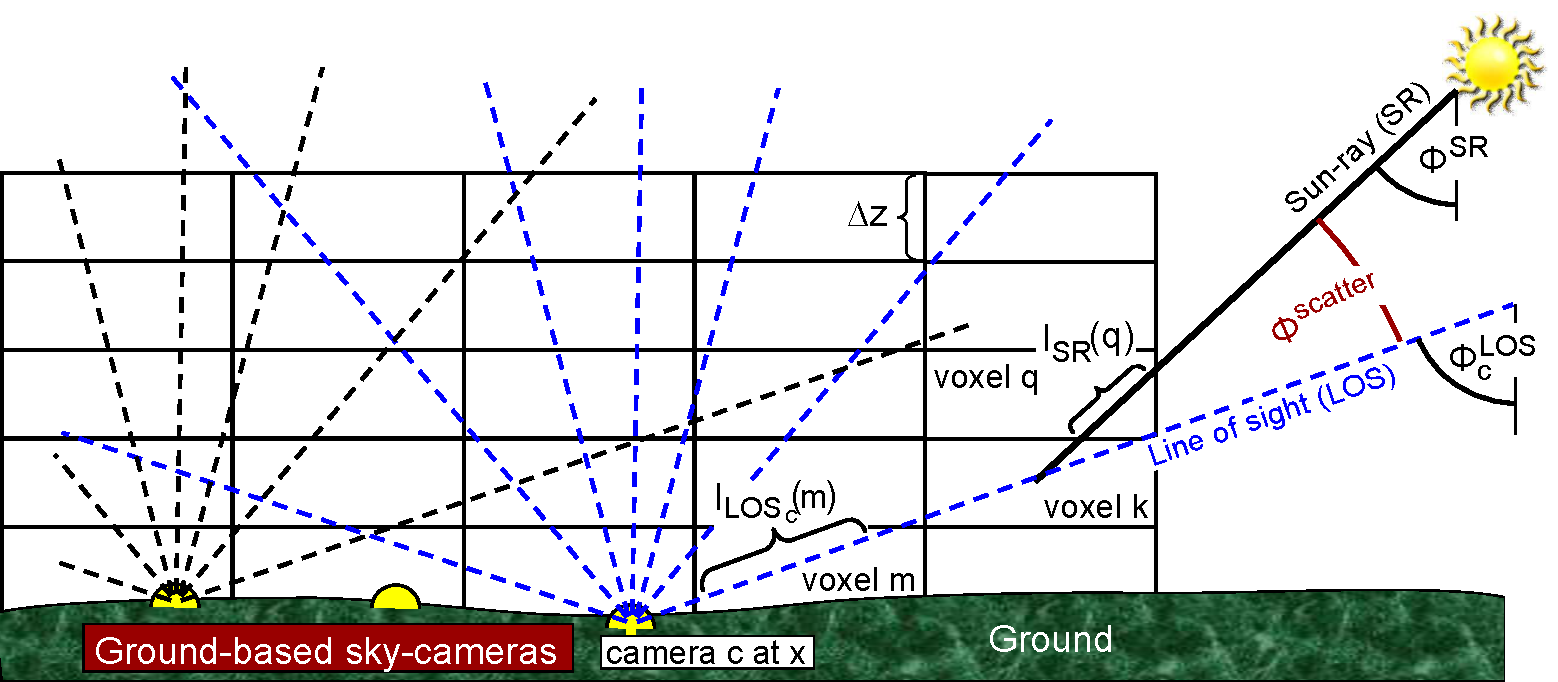
\includegraphics[width=\linewidth]{images/groundtomog24.pdf}}
  \end{center}
  \caption{\small Integral (lightfield) imaging through a volumetric
    distribution in the atmosphere, using ground-based cameras.}
  \label{fig:groundgrid}
\end{figure*}


%%%%%%%%%%%%%%%%%%%%%%%%%%%%%%%%%%%%%%%%%%%%%%%%%%%%%%%%%%%%
%%%%%%%%%%%%%%%%%%%%%%%%%%%%%%%%%%%%%%%%%%%%%%%%%%%%%%%%%%%%

\section{Theoretical background}
\label{sec:theor-backgr}

\noindent {\bf Extinction}: Sun rays (SR) irradiate a small volume
that includes particles of a certain type.  Each particle has an {\em
  extinction cross section} for interacting with the irradiance. An
aerosol extinction cross section is denoted $\sigma^{\rm aerosol}$.
The aerosol density is $n$. Per unit volume, the {\em extinction
  coefficient} due to aerosols is $\beta^{\rm aerosol}= \sigma^{\rm
  aerosol} n$. In addition, the atmosphere contains air molecules.
The extinction coefficient due to the molecules is $\beta^{\rm air}$.
The volume has infinitesimal length $dl$. Then, the relative portion
of extinct SR irradiance is the unitless differential optical depth,
$d\tau= (\beta^{\rm aerosol}+\beta^{\rm air}) dl$.  The {\em optical
  depth} aggregates in extended propagation:
\begin{align}
  \tau= \int d\tau=\int (\beta^{\rm aerosol}+\beta^{\rm air}) dl =\int
  (\sigma^{\rm aerosol} n +\beta^{\rm air}) dl = \tau^{\rm air}+ \int
  \sigma^{\rm aerosol} n dl \;,
  \label{eq:tau}
\end{align}
where $\tau^{\rm air}=\int \beta^{\rm air} dl$.  Through an
attenuating atmosphere, the {\em transmittance} exponentially decays
with the optical depth:
\begin{align}
  t=\exp(-\tau) \;.
  \label{eq:beer-lambert}
\end{align}

\noindent {\bf Scattering}: Interaction of a single particle with the
irradiance is by absorption and scattering. The weight of scattering
(to all directions), relative to the total extinction is given by the
unitless {\em single scattering albedo} of the particle. For an
aerosol, the single scattering albedo is denoted $\varpi^{\rm
  aerosol}$.  The {\em scattering coefficient} due to aerosols in the
volume is
\begin{align}
  \alpha^{\rm aerosol}= \varpi^{\rm aerosol}\beta^{\rm aerosol}
  =\varpi^{\rm aerosol} \sigma^{\rm aerosol} n \;.
  \label{eq:alph}
\end{align}
The angular distribution of scattering by an aerosol is determined by
a {\em phase function} $P^{\rm aerosol}$, which is normalized: its
integral over all solid angles is unit. Part of the light scatters
towards a camera's LOS, as illustrated in \cref{fig:groundgrid}. The
angle between the SR and LOS is the scattering angle $\Phi^{\rm
  scatter}$. The {\em angular scattering coefficient} due to aerosols
is
\begin{align}
  \tilde\alpha^{\rm aerosol}(\Phi^{\rm scatter}) = \alpha^{\rm
    aerosol} P^{\rm aerosol}(\Phi^{\rm scatter}) = \varpi^{\rm
    aerosol} \sigma^{\rm aerosol} n P^{\rm aerosol}(\Phi^{\rm
    scatter}).
  \label{eq:alphabasic}
\end{align}
The phase function is often approximated by a parametric
expression. Specifically, the Henyey-Greenstein~\cite{Cornette1995}
function is governed by an {\em anisotropy parameter} $g$:
\begin{align}
  P^{\rm aerosol}_g(\Phi^{\rm scatter})\approx \frac{3}{8\pi} \frac{(1 -
  g^2)(1+\mu^2)}{(2+g^2)(1 + g^2 - 2g\mu)^{\sfrac{3}{2}}}
  \label{eq:aerosol_scatter}
\end{align}
\hl{where $\mu\equiv \cos \Phi^{\rm scatter}$}

Scattering by air molecules follows the {\em Rayleigh} model. The
phase function is
\begin{align}
  P^{\rm air}(\Phi^{\rm scatter}) &\approx
  \frac{3}{16\pi}(1+\cos^2\Phi^{\rm scatter})
  \label{eq:rayleighP}
\end{align}
and the single scattering albedo in visible light is $\varpi^{\rm
  air}$=1. Air molecular density falls off approximately exponentially
with altitude $h$, with a characteristic~\cite{Levi1980} falloff
height $H^\mathrm{air}=8\ \si{\km}$. Thus, the
coefficients for extinction and scattering by air molecules can be
modeled by~\cite{Levi1980},
\begin{align}
  \alpha^{\rm air}(h, \lambda)=\beta^{\rm air}(h, \lambda) \approxeq
  1.09 \times 10^{-3}\lambda^{-4} \exp(-h/H^\mathrm{air})
  \;,%\left[-\frac{h}{H^\mathrm{air}}\right].
  \label{eq:rayleighbeta}
\end{align}
where $\lambda$ is the wavelength, in microns.
\\

\noindent {\bf Inverse transform sampling}: A tool for RT modeling is
the Monte-Carlo (MC) method. MC considers scattering and extinction as
random phenomena, that are sampled from their probability
distributions. 
Inverse transform sampling~\cite{devroye1986sample} is used for 
sampling random numbers that comply with a specified
probability density function. Let $u$ be a random number drawn
from a uniform distribution in the interval $[0,1]$. The number $u$
can be transformed into a random variable $X$, whose cumulative
distribution function (CDF) is $F(X)$. The transform is $X =
F^{-1}(u)$.

For example, consider a photon propagating in the atmosphere.  The
photon has high probability of propagating as long as $t$ is high, and
the probability diminishes as $t\rightarrow 0$. Thus
(\cref{eq:beer-lambert}) can be viewed as a probability density
function, whose CDF is
\begin{equation}
  \label{eq:Ftau}
  F(\tau)=\int_{0}^{\tau}\exp(-\tau')\derivsym{\tau'}=1-\exp(-\tau).
\end{equation}
Thus a photon propagates to a random optical depth
\begin{equation}
  \label{eq:taurand}
  \tau^{\rm random}=F^{-1}(u)=-\ln(1-u).
\end{equation}
If the atmosphere is uniform, then from \cref{eq:tau} the photon
reaches a random distance
\begin{equation}
  \label{eq:lrand}
  l^{\rm random}= (\beta^{\rm aerosol}+\beta^{\rm air})^{-1} \tau^{\rm random}
  = -(\beta^{\rm aerosol}+\beta^{\rm air})^{-1}\ln(1-u),
\end{equation}
before interacting with a particle. If the number of photons launched
is very high, their average number falls off in consistency with
\cref{eq:tau,eq:beer-lambert}.  Analogous transforms
generate scattering at random angles, according to the phase function.

%%%%%%%%%%%%%%%%%%%%%%%%%%%%%%%%%%%%%%%%%%%%%%%%%%%%%%%%%%%%
%%%%%%%%%%%%%%%%%%%%%%%%%%%%%%%%%%%%%%%%%%%%%%%%%%%%%%%%%%%%

\section{3D recovery approach and its assessment}
\label{sec:methodology}

A set of ground-based wide-angle cameras looks upwards
(\cref{fig:groundgrid}), performing {\em integral
  imaging}~\cite{Hong2004} of the sky. Per viewpoint, the view azimuth
and elevation angles (relative to the zenith and north) are
encapsulated in vector ${\bm{\Theta}}$. Any camera $c$ is at a
distinct fixed location, capturing raw image
$i_c({\bm{\Theta}})$. This paper reports a first step: formulating a
principle for estimating 3D atmospheric aerosols distributions, using
such data. To theoretically study the feasibility and cross validate
it, we perform RT using two different forward models. A forward model
takes as input a 3D aerosol distribution, and outputs images as if
captured at various viewpoints.  One model uses MC
(\cref{sec:monte-carlo-simul}): it is stochastic, slow but
naturally expresses multiple-scattering. Hence, MC rigorously
simulates realistic scenes of arbitrary complexity.
% MC simulations can be made arbitrarily accurate by increasing the
% number of launched %photons. MC methods are highly parallelizable.
The second model uses the single-scattering approximation
(\cref{sec:single-scatt-model}). It is less accurate than MC, but
solves RT in an analytic, closed form. This form enables simple
inversion of the model, to estimate the underlying aerosol
distribution (\cref{sec:inverse-problem}).

%%%%%%%%%%%%%%%%%%%%%%%%%%%%%%%%%%%%%%%%%%%%%%%%%%%%%%%%%%%%
%%%%%%%%%%%%%%%%%%%%%%%%%%%%%%%%%%%%%%%%%%%%%%%%%%%%%%%%%%%%

\section{Single-scattering forward model}
\label{sec:single-scatt-model}

As illustrated in \cref{fig:groundgrid,fig:distributions},
The sky is discretized into a grid of $N_{\rm voxels}$ \fix{volume
  elements}{rectangular cuboid elements}
(voxels), indexed by $k$, $m$ or $q$.
\begin{figure}
  \centering
  \yoavcomment{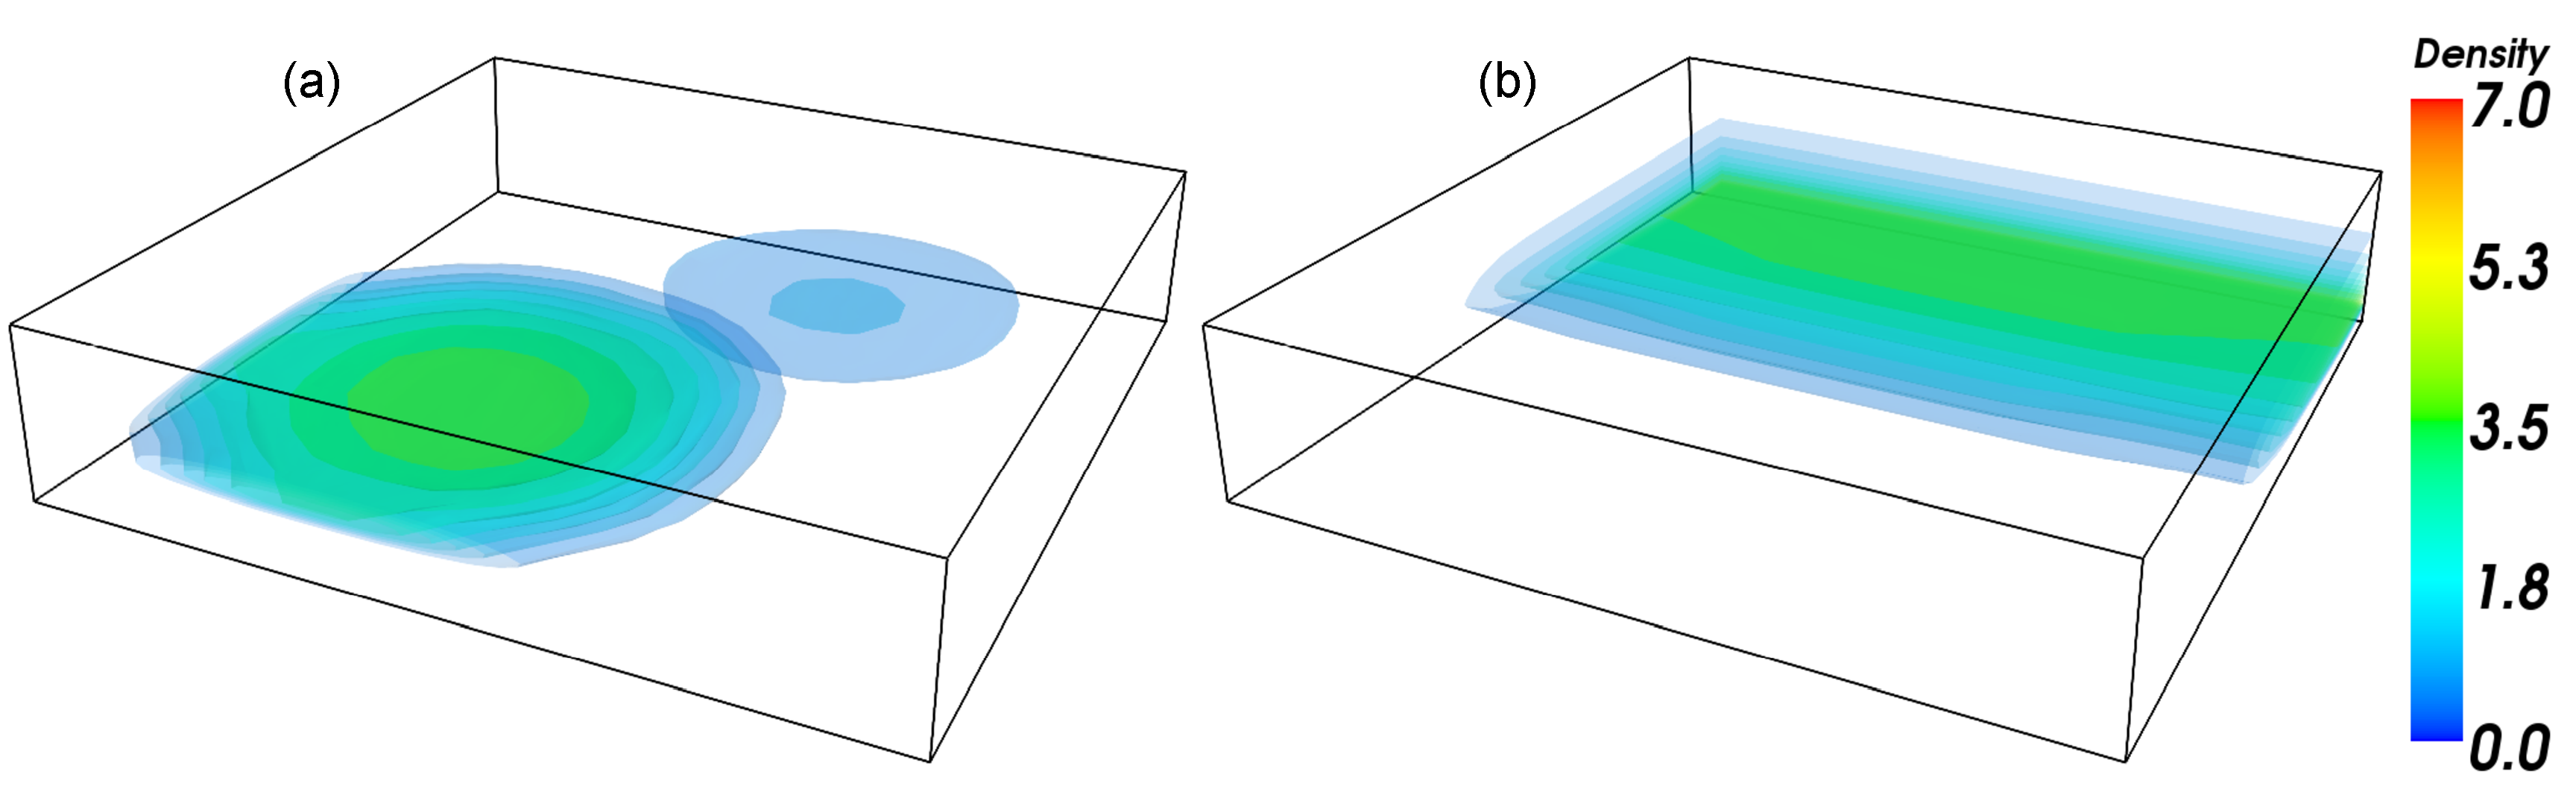
\includegraphics[width=\columnwidth]{images/distributions}}
  \caption{\small Simulated 3D aerosol distributions: [a] {\em Haze
      blobs} and [b] {\em Haze Front}.  Here, an aerosol density unit
    is $10^{6}~{\rm particles}/{\rm m}^3.$ The atmopsheric domain has
    area of $50\times 50{\rm km}^2$, extending from the ground up to
    altitude of 10km. The domain is divided into a rectilinear grid
    having $N_{\rm voxels}$ voxels.}
  \label{fig:distributions}
\end{figure}
In a \emph{single-scattering} model, any SR changes direction only
once on the way to a camera. This model is valid in atmospheres that
are not very dense: inside fog and clouds this model does not
apply. In this model, RT has three steps (\cref{fig:groundgrid}):
({\tt i}) Attenuation of a SR propagating from the top of the
atmosphere (TOA) to voxel $k$. ~({\tt ii}) Light scattering at voxel
$k$, towards a camera. ~({\tt iii}) Light attenuation on the LOS from
voxel $k$ to the camera.~~ Steps~{\tt i},{\tt iii} involve the optical
depth along the light path to and from voxel $k$, as analyzed in
\cref{sec:optical-depth}.  Step~{\tt ii} involves the scattering
coefficient at voxel $k$, described in \cref{sec:scattering}.

%%%%%%%%%%%%%%%%%%%%%%%%%%%%%%%%%%%%%%%%%%%%%%%%%%%%%%%%%%%%

\subsection{Optical depth}
\label{sec:optical-depth}

Denote a SR line segment between the TOA and the center of voxel $k$
by $[{\rm SR},k]$ (See \cref{fig:groundgrid}). This SR intersects
voxel $q$. The intersection line segment has geometric length $l_{\rm
  SR}(q|\Delta z,\Phi^{\rm SR},k)$, where $\Delta z$ is a voxel's
vertical geometric thickness, and $\Phi^{\rm SR}$ is the Sun
angle. Define a \mbox{$N_{\rm voxels}\times N_{\rm voxels}$} matrix
$\OpDistance^{\mathrm{Sun \rightarrow voxel}}$, whose element $(k,q)$
represents $l_{\rm SR}(q)$:
\begin{equation}
  \OpDistance^{\mathrm{Sun \rightarrow voxel}}(k,q) =
  \left\{
    \begin{array}{ll}
      l_{\rm SR}(q) & \mbox{ if $q \in[{\rm SR},k]$} \\
      0  & \mbox{ otherwise}
      \label{eq:Dsv}
    \end{array}
  \right.
  \hspace{-0.05cm}
\end{equation}
Matrix $\OpDistance^{\mathrm{Sun \rightarrow voxel}}$ is sparse.
Analogously, for camera $c$, denote by $[{\rm LOS}_c,k]$ a LOS bounded
between the camera and the center of voxel $k$ (see
\cref{fig:groundgrid}).  The LOS zenith angle is $\Phi^{\rm LOS}_c$.
Suppose this LOS intersects voxel $q$. The geometric length of this
intersection line segment is $l_{\rm LOS_c}(m|\Delta z,\Phi^{\rm
  LOS}_c,k)$.  As in \cref{eq:Dsv}, define a $N_{\rm voxels}\times
N_{\rm voxels}$ sparse matrix whose element $(k,m)$ is
\begin{equation}
  \OpDistance^{\mathrm{voxel \rightarrow cam}}_c(k,m) =
  \left\{
    \begin{array}{ll}
      l_{{\rm LOS}_c}(m) & \mbox{ if $m \in[{\rm LOS}_c,k]$} \\
      0  & \mbox{ otherwise}
      \label{eq:Dvc}
    \end{array}
  \right.
  .
  \hspace{-0.05cm}
\end{equation}

We focus on situations where, in addition to air molecules, there is a
single type of aerosol over a scene. Hence, the three-element vector
$[{\sigma}^{\rm aerosol},\varpi^{\rm aerosol},g]$ is uniform across
the scene, but the density distribution $n(k)$ is
variable. As a numerical approximation, assume that within any voxel,
the molecular parameters $\{ \beta^{\rm air}(k),\alpha^{\rm air}(k)\}$
and the aerosol density $n(k)$ are constants, e.g., corresponding to
the value at each voxel center.  Following \cref{eq:tau}, the optical
depths between the TOA and voxel $k$, and from voxel $k$ to camera $c$
are
\begin{align}
  \tau_{\rm SR}(k)&= \sum_{q \in[{\rm SR},k]} l_{\rm SR}(q)
  [\beta^{\rm air}(q)+\sigma^{\rm aerosol} n(q)] \nonumber \\
  \tau_{{\rm LOS}_c}(k)&= \sum_{m \in[{\rm SR},k]} l_{{\rm LOS}_c}(m)
  [\beta^{\rm air}(m)+\sigma^{\rm aerosol} n(m)].
  \label{eq:lSRn}
\end{align}
Let ${\DistUnknown}$, $\vect{\tau}_{\rm SR}$ and $\vect{\beta}^{\rm air}$ be column
stack vector representations of $n(k)$, $\tau_{\rm SR}(k)$ and $\beta^{\rm
  air}(k)$, respectively.  Then, we can write \cref{eq:lSRn} using
matrix notation: 
\begin{align}
  \vect{\tau}_{\rm SR} &= \OpDistance^{\mathrm{Sun
      \rightarrow voxel}}\vect{\beta}^{\rm air} + \sigma^{\rm
    aerosol}\OpDistance^{\mathrm{Sun \rightarrow voxel}}
  {\DistUnknown} \nonumber \\
  \vect{\tau}_{{\rm LOS}_c} &=
  \OpDistance_c^{\mathrm{voxel \rightarrow cam}}\vect{\beta}^{\rm air} +
  \sigma^{\rm aerosol}\OpDistance_c^{\mathrm{voxel \rightarrow cam}}
  {\DistUnknown}.
\end{align}

The SR and LOS paths joining at each voxel form a
single path from the TOA to camera $c$.  Hence, in matrix notation,
\cref{eq:tau} yields the total optical depths corresponding to LOSs
(of camera $c$) and SRs that cross all voxels:
\begin{equation}
  \vect{\tau}_c= \vect{\tau}_c^{\rm air}
  + \sigma^{\rm aerosol} {\bm D}_c {\bm n}
  \;\;,
  \label{eq:tautotal}
\end{equation}
where ${\bm D}_c= {\bm D}^{\mathrm{Sun \rightarrow voxel}}+ {\bm
  D}^{\mathrm{voxel \rightarrow cam}}_c$ and $\vect{\tau}_c^{\rm air}=
{\bm D}_c \vect{\beta}^{\rm air}$.
  
%%%%%%%%%%%%%%%%%%%%%%%%%%%%%%%%%%%%%%%%%%%%%%%%%%%%%%%%%%%%

\subsection{Scattering}
\label{sec:scattering}

Per camera $c$ and voxel $k$, the lines $[{\rm SR},k]$ and $[{\rm
  LOS}_c,k]$ intersect at a fixed angle $\Phi^{\rm scatter}_c(k)$.
Column-stacking all angles yields the vector representation of all
scattering angles in the domain, $\vect{\Phi}^{\rm scatter}_c$ per
camera $c$.
% Similarly, the single-scattering albdeos $\varpi^{\rm aerosol}$ in
% all voxels are stacked to vector $\vect{\varpi}$.
Using \cref{eq:alphabasic,eq:rayleighP}, the angular scattering
coefficients across the domain are expressed in vector form by
\begin{equation}
  \tilde{\vect{\alpha}}^{\rm air}_c =
  \vect{\beta}^{\rm air} \odot P^{\rm air}(\vect{\Phi}^{\rm scatter}_c)\;,
  \quad
  \tilde{\vect{\alpha}}^{\rm aerosol}_c =
  \varpi^{\rm aerosol} \sigma^{\rm aerosol}
  {\bm n} \odot P^{\rm aerosol}_{\bm g}(\vect{\Phi}^{\rm scatter}_c) \;.
  \label{eq:alpha_matrix}
\end{equation}
Here the operator $\odot$ denotes the Hadamard (element-wise) product.

%%%%%%%%%%%%%%%%%%%%%%%%%%%%%%%%%%%%%%%%%%%%%%%%%%%%%%%%%%%%

\subsection{Image capture}
\label{sec:captured-image}

Compounding the attenuation of irradiance along both $[{\rm SR},k]$
and $[{\rm LOS}_c,k]$, and scattering by voxel $k$ towards the camera
(\cref{eq:beer-lambert,eq:tautotal,eq:alphabasic}) the radiant power
contributed by the voxel is
\begin{equation}
  p_c(k)= L^{\rm TOA}
  [\tilde{\alpha}^{\rm air}_c(k) + \tilde{\alpha}^{\rm aerosol}_c(k)]
  \exp[-\tau_c(k)]
  \;\;,
  \label{eq:ick}
\end{equation}
where $L^{\rm TOA}$ is the radiance at the TOA. A column-stack vector
of all voxel contributions is
\begin{equation}
  {\bm p}_c= L^{\rm TOA}
  (\tilde{\vect{\alpha}}^{\rm air}_c + \tilde{\vect{\alpha}}^{\rm aerosol}_c)
  \odot \exp(-\vect{\tau}_c)
  \;\;.
  \label{eq:pc}
\end{equation}

A camera sensor comprises $N_{\rm pix}$ pixels. Each pixel collects light from a narrow cone in the
atmosphere. The cone contains or intersects some voxels, while being
oblivious to all the rest.  Overall, light power captured at the pixel
is a weighted sum of the power $p_c(k)$ radiating from all voxels.  This sum is
formulated by a matrix operation ${\vect{\Pi}}_c$ over ${\bm p}_c$:
\begin{equation}
  {\bm i}_c= {\vect{\Pi}}_c{\bm p}_c
  \;\;,
  \label{eq:IcP}
\end{equation}
where ${\bm i}_c$ is the image, column-stacked to a vector $N_{\rm
  pix}$ long.  Combining
\cref{eq:tautotal,eq:pc,eq:IcP,eq:alpha_matrix}, the captured image is thus
\begin{align}
  {\bm i}_c= L^{\rm TOA} {\vect{\Pi}}_c \left\{
  \left[\tilde{\vect{\alpha}}^{\rm air}_c + \varpi^{\rm aerosol}\sigma^{\rm
    aerosol} P^{\rm aerosol}_g(\vect{\Phi}^{\rm scatter}_c) \odot{\bm
    n} \right] \odot \exp\left[-(\vect{\tau}_c^{\rm air} + {\sigma}^{\rm aerosol}
  {\bm D}_c{\bm n})\right] \right\} .
  \label{eq:bigIA}
\end{align}

%%%%%%%%%%%%%%%%%%%%%%%%%%%%%%%%%%%%%%%%%%%%%%%%%%%%%%%%%%%%
%%%%%%%%%%%%%%%%%%%%%%%%%%%%%%%%%%%%%%%%%%%%%%%%%%%%%%%%%%%%

\section{Examples}
\label{sec:simul}

\begin{figure}
  \centering
  \yoavcomment{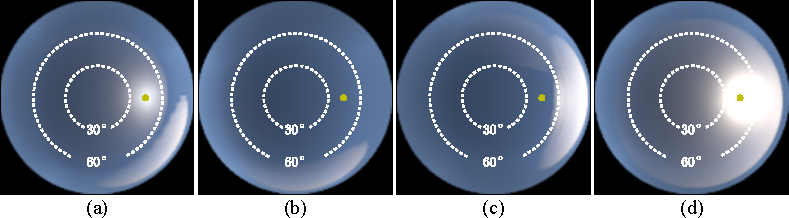
\includegraphics[width=\linewidth]{images/single_images.pdf}}
  \caption{\small Different viewpoints of a sky that includes {\em
      Haze Blobs}. Images are rendered using the single-scattering model.
    A yellow dot marks the Sun location. Dashed white circles mark
    zenith angles.}
  \label{fig:simulation-results1}
\end{figure}
To demonstrate the model, we simulated some scenarios, whose details are as follows.
\\

\noindent{\bf Geometry}: The sun is at zenith angle $\Phi^{\rm
  SR}=45^o$.  Its $L^{\rm TOA}$ is obtained
from~\cite{BBradiance,sun_composition}, with respective red-green-blue
ratios of $L^{\rm TOA}_{\rm R}:L^{\rm TOA}_{\rm G}:L^{\rm TOA}_{\rm
  B}=255:236:224$.

The atmospheric domain is described in \cref{fig:distributions}.
We tested domain division to various grids, from $10\times10 \times
20$ voxels, up to $50\times50 \times 100$. The corresponding voxels
had width, length and thickness of $5{\rm km}\times 5{\rm km} \times
0.5{\rm km}$ and $1{\rm km}\times 1{\rm km} \times 0.1{\rm km}$.  Each
ground-based camera has a hemispherical field of view, and low
resolution, $128 \rm{px} \times 128 \rm{px}$, as cloudless (yet hazy)
sky images are rather smooth.
\\

\noindent{\bf Aerosol}: We used particle-type 6 from the aerosol list
in~\cite{Martonchik2009}. This is a spherical non-absorbing
sea-salt/organic particle, whose anisotropy parameter per color
channel is $[g_{\rm R},g_{\rm G},g_{\rm B}]=[0.763,0.775,0.786]$. Its
corresponding extinction cross sections are $[\sigma^{\rm
  aerosol}_{\rm R}, \sigma^{\rm aerosol}_{\rm G}, \sigma^{\rm
  aerosol}_{\rm
  B}]=[16.5,16.2,15.9]$~\si[sticky-per]{\per\micro\meter\squared}.  At
all channels, $\varpi^{\rm aerosol}=1$. We simulated spatial
distributions using a product of two functions. To express the general
trend of reduced density with altitude $h(k)$ of voxel $k$, we
follow~\cite{Levi1980} and set the first function as
\begin{align}
  f_1[h(k)] = n^{\rm sealevel}
  \exp[-h(k)/H^\mathrm{aerosol}],
\end{align}
where $H^\mathrm{aerosol}=2$~\si{\km}. To express a clustered nature
of aerosol distributions (as clouds), we define blobs in the form of
3D ellipsoids. There may be multiple ellipsoids suspended.  Then
\begin{equation}
  f_2(k) =
  \left\{
    \begin{array}{ll}
      1  & \mbox{ if $k\in$ any blob cluster} \\
      0  & \mbox{ otherwise}
      \label{eq:f2}
    \end{array}
  \right.
  .
  \hspace{-0.05cm}
\end{equation}
The true aerosol distribution is then ${\bm n}^{\rm true}={\cal
  S}\{{\bm f}_1\odot {\bm f}_2\}$, where ${\cal S}$ is 3D spatial
smoothing, obtained by narrow 3D Gaussian filtering. It expresses
non-sharp boundaries of typical distributions. The {\em Haze Blobs}
scene in \cref{fig:distributions}(a) uses two ellipsoids: one is 32km
wide, 2.8km thick and centered at altitude 2.5km; the other is 24km
wide, 2.1km thick and centered at altitude 5km. Horizontal widths
are much larger than the vertical thickness, in consistency with
atmospheric scales. \Cref{fig:simulation-results1} shows
photographs of the {\em Haze Blobs} scene, as simulated by
\cref{eq:bigIA}.

The {\em Haze Front} scene in \cref{fig:distributions}(b) uses an
ellipsoid degenerated to an elliptic cylinder that partly enters the
analyzed volume. It is 32km long (only part of which enters the
volume), 4km thick and centered at altitude 5km. The front stretches
across the domain width.
%%%%%%%%%%%%%%%%%%%%%%%%%%%%%%%%%%%%%%%%%%%%%%%%%%%%%%%%%%%%
%%%%%%%%%%%%%%%%%%%%%%%%%%%%%%%%%%%%%%%%%%%%%%%%%%%%%%%%%%%%

\section{Multiple-scattering forward model by Monte Carlo}
\label{sec:monte-carlo-simul}


The MC simulations rely on the same grid as
\cref{sec:single-scatt-model}. We use backward MC: from a detector
pixel, photons are `launched' via the camera lens; then the photons
are traced back through the atmosphere. Photons that happen to be
back-traced to the Sun are counted, per pixel. In this model, RT takes
the following steps, per pixel (\cref{fig:mcgrid}(a)):
\begin{figure}
  \centering
  \yoavcomment{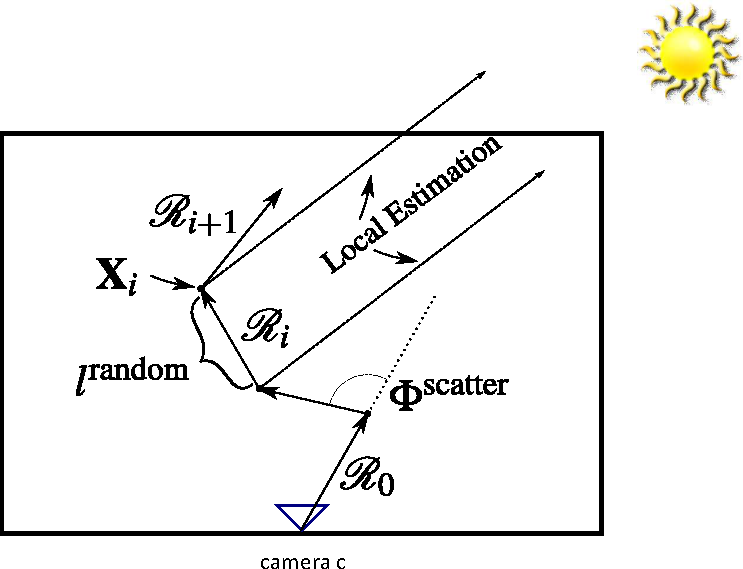
\includegraphics{images/mcgrid.pdf}}
  \caption{\small [a] Multiple-scattering forward model by MC.
    [b] Photograph of the same sky and view point as in
    \cref{fig:simulation-results1}[left], rendered using MC.}
  \label{fig:mcgrid}
\end{figure}

\noindent ({\tt i}) Launch a photon-packet from camera $c$ to
direction ${\bm{\Theta}}$. This is the initial {\em ray}, denoted
${\cal R}_0$. The packet has intensity $I_0$.

\noindent Per iteration $i$:

\noindent ({\tt ii}) Find the distance on ray ${\cal R}_{i}$ to which
the photon-packet propagates. To do this, \cref{eq:taurand}
yields $\tau^{\rm random}$. Then, \cref{eq:lrand} generalizes to
a non-uniform atmosphere: using \cref{eq:tau}, numerically seek
$l^{\rm random}$ s.t.
\begin{align}
  \int_0^{l^{\rm random}}(\sigma^{\rm aerosol} n +\beta^{\rm air}) dl
  = \tau^{\rm random}
  \label{eq:MCextinct}
\end{align}
Distance $l^{\rm random}$ along ${\cal R}_{i}$ yields the 3D position ${\bf
  X}_{i}$.  If ${\bf X}_{i}$ is outside the atmospheric grid, the
packet is terminated. If, in addition, ${\cal R}_{i}\parallel {\rm
  SR}$ , the packet is counted as contributing to the image pixel.

\noindent ({\tt iii}) The type of particle (air molecule or aerosol)
that the photon-packet interacts with at point ${\bf X}_{i}$ is determined
randomly according to their relative densities at the voxel containing
${\bf X}_{i}$.

\noindent ({\tt iv}) If it is an aerosol, the photon-packet intensity
is attenuated to $I_{i+1}=\varpi^{\rm aerosol}I_{i}$. If $I_{i+1}$ is
lower than a threshold, the packet is stochastically terminated,
following~\cite{Iwabuchi2006}.

\noindent ({\tt v}) The photon-packet is scattered to a new direction,
determined by inverse transform sampling, according to the phase
function of the particle (Eqs.~(\ref{eq:aerosol_scatter})
or~(\ref{eq:rayleighP})). This yields a new {\em ray}, denoted ${\cal
  R}_{i+1}$, emanating from ${\bf X}_{i}$. Local
Estimation~\cite{marshak20053d} is used for calculating the amount of
light back-traced to the sun at each scattering. The next iteration of
propagation (denoted {\tt ii} above) proceeds.

The quality of MC increases with the number of photons launched.
\Cref{fig:mcgrid}(b) shows a photograph of the {\em Haze Blobs}
scene, derived by the MC process, using \num{10000} photons per pixel,
from the same viewpoint as \cref{fig:simulation-results1}[left].
Comparison of \hl{horizontal and vertical cross sections along 
matching MC and single-scattering simulated images are} shown in
\cref{fig:cross_sections}(a) and \cref{fig:cross_sections}(b).
\hl{The cross sections indicate fair correspondence between
the MC and single-scattering simulations.}
\begin{figure}[th]
  \centering
  \yoavcomment{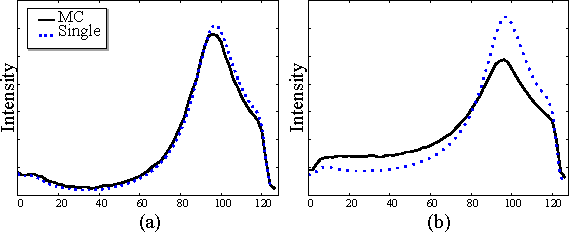
\includegraphics{images/cross_sections.pdf}}
  \caption{\small Cross sections along the $X$-Axis [a] and $Y$-Axis [b] of
    a MC and single-scattering simulations. Overlay of the cross
    sections on the MC simulated image is shown in [c]. }
  \label{fig:cross_sections}
\end{figure}

\Cref{fig:scatter_order} \hl{shows the contribution of subsequent
scattering events to the MC image. The amount of light scattered
in the direction of the sun due to the first scatter event of each photon
is collected to create} \cref{fig:scatter_order}(a). \hl{This process
is repeated for the second and third scatter events creating}
\cref{fig:scatter_order}(b) and \cref{fig:scatter_order}(c),
\hl{respectively. It is conspicuous that the first scatter is responsible
for most of the energy in the MC image. The effect of subsequent scatters
is mostly evident at the horizon. The line of sight extending into the
horizon crosses a larger volume of atmosphere then the line of sight extending
in the direction of the zenith. This increases the probability of
scattering events along the line of sight extending into the horizon.}
\begin{figure}[h]
  \centering
  \yoavcomment{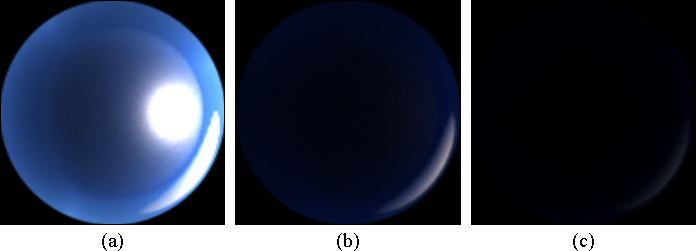
\includegraphics{images/scatter_order.pdf}}
  \caption{\small Separation of a MC simulated image to (a) first
   scattering order, (b) second scattering order and (c) third
   scattering order. }
  \label{fig:scatter_order}
\end{figure}

%%%%%%%%%%%%%%%%%%%%%%%%%%%%%%%%%%%%%%%%%%%%%%%%%%%%%%%%%%%%
%%%%%%%%%%%%%%%%%%%%%%%%%%%%%%%%%%%%%%%%%%%%%%%%%%%%%%%%%%%%

\section{Inverse Problem}
\label{sec:inverse-problem}

When the type of aerosol above an area is known~\cite{Martonchik2009},
estimation of the density distribution $\DistUnknown$ is needed. The
data are $N_{\rm views}$ measured photographs $\{ {\bm i}^{\rm
  measured}_c\}_{c=1}^{N_{\rm views}}$. Recovery is phrased as
optimization of a cost function that fits the image-formation model to
the data. Let $\DistSet$ be the set of all distributions complying
with some constraints.  Particularly, $\DistUnknown$ is non-negative,
and its spatial support is bounded between the ground and the TOA. The
optimization problem is
\begin{equation}
  \label{eq:minobjectiveA}
  \DistEstimated =
  \argmin_{\DistUnknown \in \DistSet} \CostFunc{\DistUnknown}
\end{equation}
where
\begin{equation}
  \label{eq:objectiveA}
  \CostFunc{\DistUnknown}
  = \sum_{c=1}^{N_{\rm views}}
  \left\|
    \MaskSun[{\bm i}^{\rm measured}_c - {\bm i}_c({\bm n})]
  \right\|^2_2  + \eta \Psi({\bm n}).
\end{equation}
Here $\MaskSun$ masks the area around the sun, as in real-world images
it is indeed blocked. \hl{It is also used for masking the areas in the image
prone for multiple scattering events, e.g. the horizon area as evident in}
\cref{fig:scatter_order}(b).  In \cref{eq:objectiveA}, $\Psi({\bm n})$
is a regularization term that expresses some prior knowledge on the
distribution, while $\eta$ is the regularization weight.

Since aerosol distributions are usually fuzzy, useful regularization
is by a {\em smoothness term}, which penalizes for energy in the second order
spatial derivatives (3D Laplacian), $\| \nabla^2{\bm
  n}\|^2_2$. Regularization is not required when data is sufficient
and reliable. As seen in \cref{fig:groundgrid}, voxels at high
altitude have good coverage by many cameras at multiple directions,
while low altitude voxels are mainly observed by local
cameras. Hence, regularization can be weakened with altitude. We
accomplish this weakening using a weight
$w(k)=\exp\left[-h(k)/H^\mathrm{smooth}\right]$.  Overall we use
\begin{equation}
  \label{eq:regularizer}
  \Psi({\bm n}) = \| {\bf W} \Laplacian{\bm n}\|^2_2
\end{equation}
where $\Laplacian$ is a matrix representation of the 3D Laplacian
operator, and matrix ${\bf W}$ is diagonal, whose elements are $w(k)$.

We solve~\cref{eq:minobjectiveA} using standard optimization tools.
The gradient of $E$ with respect to ${\bm n}$ is
\begin{align}
  \Grad{{\bm n}} E = -2\sum_{c=1}^{N_{\rm views}}
  \transpose{\left[{\bm J}_{{\bm i}_c}({\bm n})\right]} [{\bm i}^{\rm
    measured}_c - {\bm i}_c({\bm n})] + 2 \eta
  \transpose{\Laplacian}\transpose{{\bf W}}{\bf W}\Laplacian{\bm n}
  \;.
  \label{eq:gradient1}
\end{align}
Here the matrix ${\bm J}_{{\bm i}_c}({\bm n})$ is the Jacobian of the
vector ${\bm i}_c$ with respect to ${\bm n}$.  Element $(\Theta,k)$ of
the Jacobian differentiates the intensity in pixel ${\bm \Theta}$ (in
viewpoint $c$) with variation of the aerosol density at voxel $k$,
i.e., $\partial i_c({\bm \Theta})/\partial{n(k)}$.

We now detail the derivation of the Jacobian ${\bm J}_{{\bm i}_c}({\bm
  n})$. First, we provide some results relating to differentiation.
Let $\vect{a}(\vect{n}),\vect{u}(\vect{n})$ be vector functions: each
outputs a vector of length $r$. Let $\mat{C}$ be a $r \times N_{\rm
  voxels}$ matrix, where $N_{\rm voxels}$ is the length of ${\bm n}$.
Then,
\begin{align}
  \label{eq:partial1}
  \PartDeriv{\transpose{\mat{C}} (\vect{a} \odot \vect{u})}{\vect{n}}
  = \left[ \PartDeriv{\vect{a}}{\vect{n}} \OpDiag{\vect{u}} +
    \PartDeriv{\vect{u}}{\vect{n}} \OpDiag{\vect{a}} \right] \mat{C}.
\end{align}
Here $\OpDiag{\vect{v}}$ is a conversion of a general vector
$\vect{v}$ into a diagonal matrix, whose main diagonal elements
correspond to the elements of $\vect{v}$. Now, let
% \begin{align}
$\vect{a}(\vect{n}) = \exp(-{\mat{C}}\vect{n})$,
% \label{eq:example1}
% \end{align}
% In \cref{eq:example1},
where the exponent is element-wise (not raising an operator to some
power). Then
\begin{align}
  \label{eq:partial2}
  \PartDeriv{\vect{a}}{\vect{n}} &= - \transpose{\mat{C}} \,
  \OpDiag{\exp(-{\mat{C}}\vect{n})}.
\end{align}
Using \cref{eq:partial2},
\begin{align}
  \label{eq:partial4}
  \PartDeriv{\exp[-(\vect{\tau}_c^{\rm air} + {\sigma}^{\rm
      aerosol}{\bm D}_c {\bm n})]}
  {\vect{n}} &= - {\sigma}^{\rm aerosol}\transpose{\OpDistance_c} \,
  \OpDiag{\exp[-(\vect{\tau}_c^{\rm air} + {\sigma}^{\rm aerosol}{\bm
      D}_c {\bm n})]},
\end{align}
where $\vect{\tau}_c^{\rm air}$ is independent of ${\bm n}$. Using
\cref{eq:partial1},
\begin{align}
  \label{eq:partial3}
  \PartDeriv{\, [\varpi^{\rm aerosol}\sigma^{\rm aerosol} P^{\rm
      aerosol}_g(\vect{\Phi}^{\rm scatter}_c) \odot{\bm n}]}{\vect{n}}
  = \varpi^{\rm aerosol}\sigma^{\rm aerosol}\OpDiag{P^{\rm
      aerosol}_g(\vect{\Phi}^{\rm scatter}_c)}.
\end{align}
Based on \cref{eq:partial4,eq:partial1,eq:partial3},
we derive the Jacobian of \cref{eq:bigIA} in close-form,
\begin{align}
  % {\bm J}_{{\bm i}_c}({\bm n}) &= L^{\rm
  % TOA}(\abbrev{A}-\abbrev{B})\abbrev{C}
  {\bm J}_{{\bm i}_c}({\bm n}) &= L^{\rm TOA}{\sigma}^{\rm
    aerosol}({\bf A}-{\bf B}) \OpDiag{\exp[-(\vect{\tau}_c^{\rm air} +
    {\sigma}^{\rm aerosol} {\bm D}_c {\bm n})]}
  \transpose{{\vect{\Pi}}_c} ,
  \label{eq:gradient2}
\end{align}
where
\begin{equation}
  \label{eq:gradient3}
  {\bf A} = \varpi^{\rm aerosol}
  \OpDiag{ P_g^{\rm aerosol}(\vect{\Phi}^{\rm scatter}_c)}
  ,\;\;\;
  {\bf B} = \transpose{{\bm D}_c}
  \OpDiag{[\tilde{\vect{\alpha}}^{\rm air}_c + \varpi^{\rm
      aerosol}\sigma^{\rm aerosol} P^{\rm aerosol}_g(\vect{\Phi}^{\rm
      scatter}_c) \odot{\bm n}    ]}
\end{equation}

%%%%%%%%%%%%%%%%%%%%%%%%%%%%%%%%%%%%%%%%%%%%%%%%%%%%%%%%%%%%
%%%%%%%%%%%%%%%%%%%%%%%%%%%%%%%%%%%%%%%%%%%%%%%%%%%%%%%%%%%%

\section{Results}
\label{sec:optimization-results}

\Cref{sec:simul} describes simulated scenes at various grid
resolutions.  Depending directly on the area grid finesse, $N_{\rm
  views}$ varied from 12 to 100.
\begin{figure}[h]
  \centering
  \yoavcomment{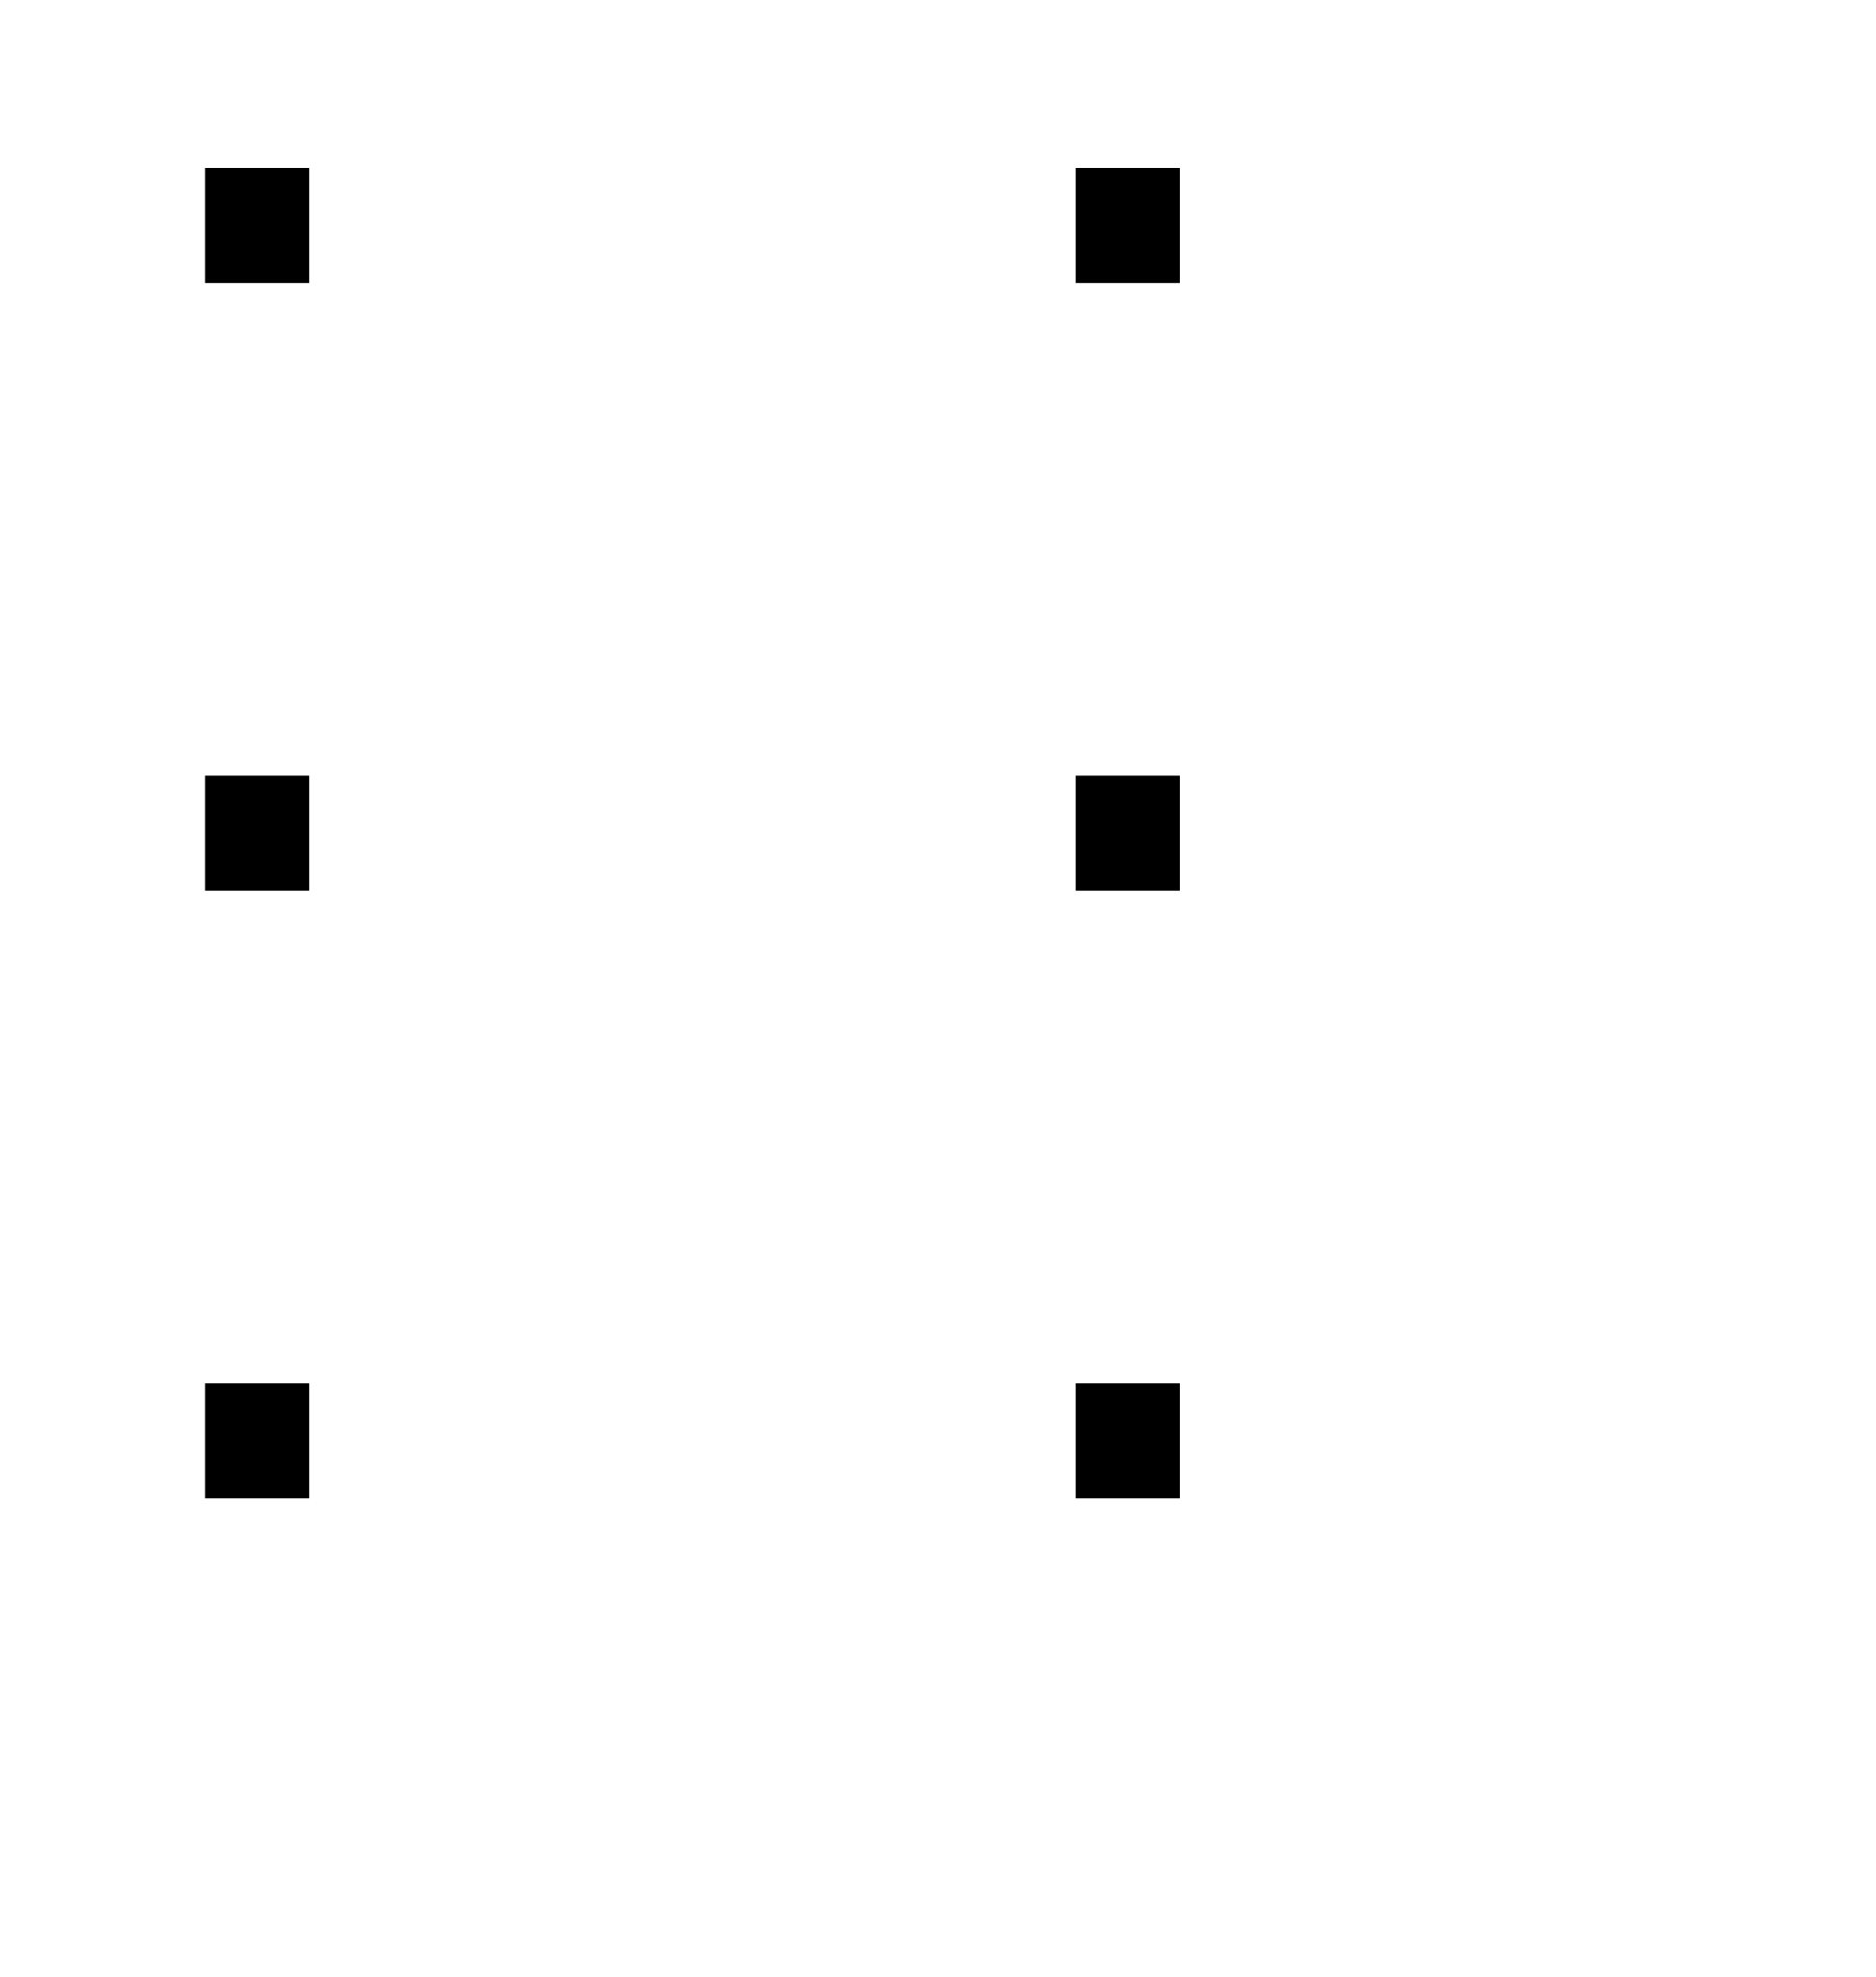
\includegraphics[width=\columnwidth]{images/results}}
  \caption{\small Reconstructions of the scenes shown in
    \cref{fig:distributions}. Color represents aerosol density. The
    density units are $10^{6}~{\rm particles}/{\rm m}^3.$ In [a,b],
    single-scattering simulated images are used as input to the
    recovery.  In [c,d], MC simulated images are used as input for the
    recovery.  }
  \label{fig:results}
\end{figure}
We applied the reconstruction algorithm to images created as described
in \cref{sec:simul,sec:monte-carlo-simul}. We used the
L-BFGS-B algorithm~\cite{BFGS} on a computer cluster. Each core was
dedicated to rendering a modeled image. The algorithm was initialized
by ${\bm n}=0$.  Satisfactory convergence occurred in several hundred
iterations. Depending on the resolution it took between minutes to a
couple of hours to complete, in total.

\Cref{fig:results} shows estimation results, corresponding to the
original distributions of \cref{fig:distributions}. 
\hl{
In these simulations the atmosphere domain was defined over a
$20\times20 \times 40$ grid. Thirty six cameras were placed
$\sim7$km apart on a $6\times6$ grid.
}
In Figs.~\ref{fig:results}(a) and (b), the single-scattering model was
used both
in rendering of the raw images, and in the estimation algorithm. In
Figs.~\ref{fig:results}(c) and (d), the MC model (multiple scattering)
rendered the raw images, over which the estimation algorithm
ran. Overall, the distributions, the density order of magnitude and
values are consistent.
Errors in Figs.~\ref{fig:results}(a) and (b) stem from random noise, which had
been induced in the raw images. Errors are larger when MC is used to
render the images, since high-order scattering is not accounted for in
the algorithm of \cref{sec:inverse-problem}. The total estimation
error can be quantified by the aerosol mass that is over and under-estimated
in all voxels, relative to the total aerosol mass in the scene. Using the $\ell_1$ norm, 
the total mass relative difference is
$(\|\hat{\bm n}\|_1 - \|{\bm n}^{\rm true} \|_1) / \| {\bm n}^{\rm true} \|_1$.
The overall mass is recovered, but for 6.5\% loss. For local errors,
 $\epsilon=\|
\hat{\bm n} - {\bm n}^{\rm true} \|_1 / \| {\bm n}^{\rm true} \|_1$.
  In Figs.~\ref{fig:results}(a) and (b), respectively $\epsilon=0.14$ and
$\epsilon=0.20$.  In Figs.~\ref{fig:results}(c) and (d), both cases have
$\epsilon=0.65$.

\hl{Optimal placement of cameras is an important aspect in realization
of the suggested system. As a first step we would like to measure the effect of
the distance between the cameras on the estimation quality. For this, we
repeated the reconstruction algorithm, each time using a subset of varying size
of the raw images. In each test the reconstruction algorithm was applied to $n_{views}$
($<N_{views}$) images. The images were selected randomly from the total $N_{views}$ raw images.
To eliminate the effect of incidental camera position, the test was repeated several
times each time with a different $n_{views}$ subset.} \Cref{fig:error_vs_cameras}
\hl{summarizes the results of these tests. In can be seen that a good estimation
is achieved already when using $20$ cameras. Over an area of $50\times 50{\rm km}^2$,
this quantity relates to placing the cameras $\sim11$km apart.}
\begin{figure}[h]
  \centering
  \yoavcomment{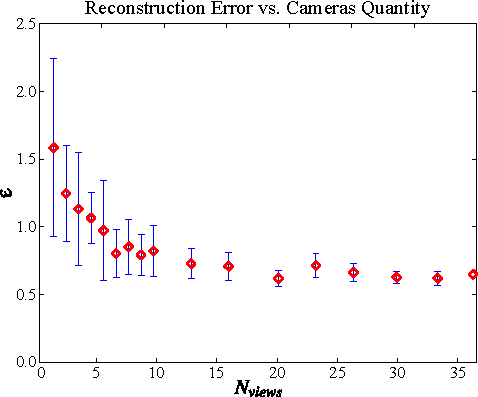
\includegraphics{images/error_vs_cameras.pdf}}
  \caption{\small Local error measure as function of cameras
    quantity. The blue error bars represent the error standard
    deviation. The dashed horizontal line marks the reconstruction
    error when all thirty six cameras are used.}
  \label{fig:error_vs_cameras}
\end{figure}

\hl{Thickening the aerosols density ten folds in the} {\em Haze Blobs} \hl{scene
resulted in a larger local error, i.e. $\epsilon=0.98$ (compared to $\epsilon=0.65$).
This admits to the fact that the single-scattering model, on which the reconstruction
algorithm is based, is valid when the optical depth of the medium is small.}
% \begin{figure}[h]
%   \centering
%   \yoavcomment{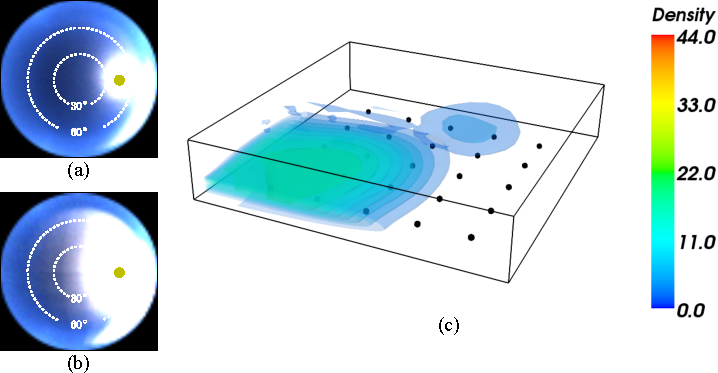
\includegraphics{images/high_density_results.pdf}}
%   \caption{\small (a) and (b) show MC simulations of low and 
%     high density scenes, respectively. (c) shows the reconstruction of
%     the high density scene.}
%   \label{fig:high_density}
% \end{figure}

%%%%%%%%%%%%%%%%%%%%%%%%%%%%%%%%%%%%%%%%%%%%%%%%%%%%%%%%%%%%
%%%%%%%%%%%%%%%%%%%%%%%%%%%%%%%%%%%%%%%%%%%%%%%%%%%%%%%%%%%%

\section{Discussion}
\label{sec:conclusions}

We describe a way to sense the 3D atmosphere. It can help remote
sensing departing from common 1D aerosol distribution models, in favor
of detailed 3D RT analysis.  The paper describes both a novel data
acquisition system concept for this recovery task (ground-based camera
network), and a dedicated algorithm for reconstructing aerosol
distributions. Using more prior knowledge on the nature of
distributions will improve the recovery.  The estimation algorithm
uses a single scattering model. This approximation is valid when the
optical depth is small. However, as the MC simulation show, it is
important to generalize this algorithm so that it explicitly
incorporates high-order scattering in the scene, including the
ground. This will certainly be needed for dense distributions as
clouds. \Cref{fig:scatter_order}(b) \hl{suggests that incorporating
the second order of scattering might be sufficient for most situations.}

To deploy such a system on a very large scale will require a long-term
engineering effort. Camera specifications~\cite{Pust2011} should be
set to optimally recover a wide range of aerosol distributions.
\hl{The relation between the quantity and spatial distribution of
  cameras and the quality of reconstruction should also be determined.}
\fix{This requires}{These open questions require} a major theoretic
 and numerical research.

%%%%%%%%%%%%%%%%%%%%%%%%%%%%%%%%%%%%%%%%%%%%%%%%%%%%%%%%%%%%
%%%%%%%%%%%%%%%%%%%%% Acknowledgments %%%%%%%%%%%%%%%%%%%%%
%%%%%%%%%%%%%%%%%%%%%%%%%%%%%%%%%%%%%%%%%%%%%%%%%%%%%%%%%%%%

\section*{Acknowledgments}
\label{sec:acknowledgments}

We thank David~J. Diner for useful discussions. Yoav Schechner is a
Landau Fellow - supported by the Taub Foundation. This work was
conducted in the Ollendorff Minerva Center. Minerva is funded through
the BMBF. Part of this work was performed at the Jet Propulsion
Laboratory, California Institute of Technology, under contract with
NASA.

\end{document}

